\subsubsection{Dama-Gruppe}\label{sec:DAM-Gr}

Die Dama-Gruppe bildet die rezente schnitzrouletteverzierte Keramik des oberen \mbox{Ubangi} ab. Die Herstellung von Gefäßen dieser Gruppe wurde 1985 durch das \textit{River Reconnaissance Project} an der namensgebenden Fundstelle Dama~I (Fpl.~222) sowie in Boduna (Fpl.~225) und Sidi (Fpl.~228) beobachtet.\footnote{Die starken Ähnlichkeiten der Keramik aus Dama~I zu jener aus Sidi wurden bereits während der Befahrung des \mbox{Ubangi} registriert. Neben den formalen Entsprechungen wies Eggert in seinem Feldbuch (29.\,08.\,1985), ausgehend von einem Hinweis von C. Kanimba Misago, auf die ähnliche Herstellungstechnik hin. An beiden Orten erfolgt die Ausformung des Gefäßkörpers in einer kleinen Erdmulde mittels eines Stempels. Siehe Anm.~\ref{ftn:EthnoToepfereiInVorb}.} Die Beschreibung der Stilgruppe gründet auf 33~GE von 15 Fundstellen aus einem relativ großen Verbreitungsgebiet, dass von Bousoka-Mangombe (Fpl.~200) im Süden bis Kouango (Fpl. 229) im Norden reicht (Abb.~\ref{fig:DAM_Verbreitung}). Charakteristika der Stilgruppe sind runde Böden, geschlossene Gefäße mit geschweifter Wandung sowie lediglich aus einem horizontalen Schnitzroulette-Band bestehende Verzierungen (Abb.~\ref{fig:DAM_Typvertreter}). Mit Ausnahme einer im Zuge der Untersuchung des Befundes MLB~85/1-3-1 (Kat.-Nr.~1) in Maluba am Lua (Fpl.~230) gefundenen GE stammen alle Funde aus Absammlungen rezenter Dorfflächen oder wurden als Ethnographica angekauft. Die Inventare der Dama-Gruppe setzen sich vor allem aus Randscherben (60\,\%) zusammen, weisen aber auch insgesamt fünf vollständige Gefäße auf. Letztere wurden am eponymen Fundort Dama~I am \mbox{Ubangi} (Fpl.~222) angekauft.

\begin{figure*}[tb]
	\centering
	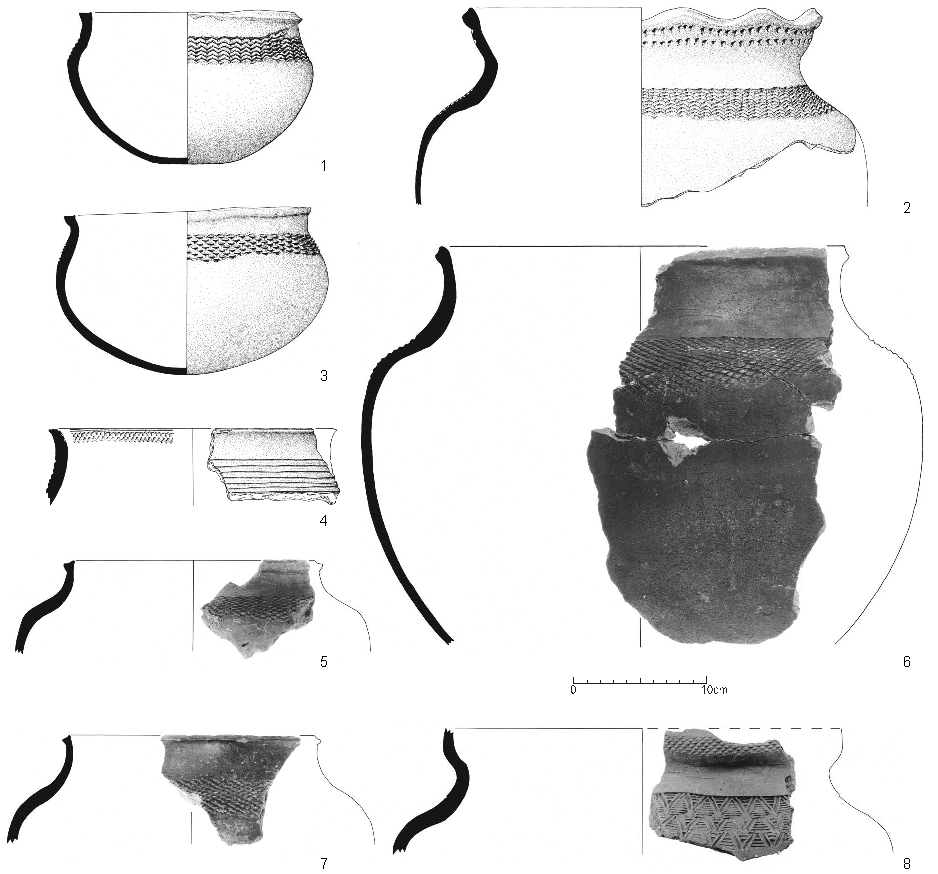
\includegraphics[width=\textwidth]{fig/DAM-Typen.pdf}
	\caption{Dama-Gruppe: Typvertreter.\\1:~Taf.~22.3; 2:~Taf.~24.1; 3:~Taf.~22.2; 4:~Taf.~12.16; 5:~Taf.~23.8; 6:~Taf.~22.4; 7:~Taf.~23.6; 8:~Taf.~23.5.}
	\label{fig:DAM_Typvertreter}
\end{figure*}

\paragraph{Technologische Merkmale}\hspace{-.5em}|\hspace{.5em}%
Die Scherben der Dama-Gruppe zeichnen sich durch ihre hohen Anteile nichtplastischer Partikel aus. Es handelt sich vornehmlich um heterogene Mischungen aus Quarzsand, in einigen Fällen wurde auch ausgebrannte Organik, Glimmer und Laterit beobachtet. Die Partikel sind ausschließlich den Größenklassen \textit{medium} (19\,\%), \textit{coarse} (32\,\%) sowie \textit{very coarse} (48\,\%) zuzurechnen. Nur wenige der Stücke (17\,\%) deuten die Nutzung weißbrennender Tone an, während ein größerer Teil eine rote Brennfarbe des Tons (34\,\%) anzeigt. Beim Gros der GE (49\,\%) ließ sich aufgrund der beigen oder grauen Färbung nicht direkt auf die Brennfarbe des genutztes Tones schließen. Die Oberflächen der meisten Scherben sind glatt (82\,\%). Nur sehr wenige Stücke zeigen eine leicht raue Oberfläche. Die Wandungsdicke der Scherben liegt im Mittel bei 7,6\,mm.

\begin{figure*}[p]
	\centering
	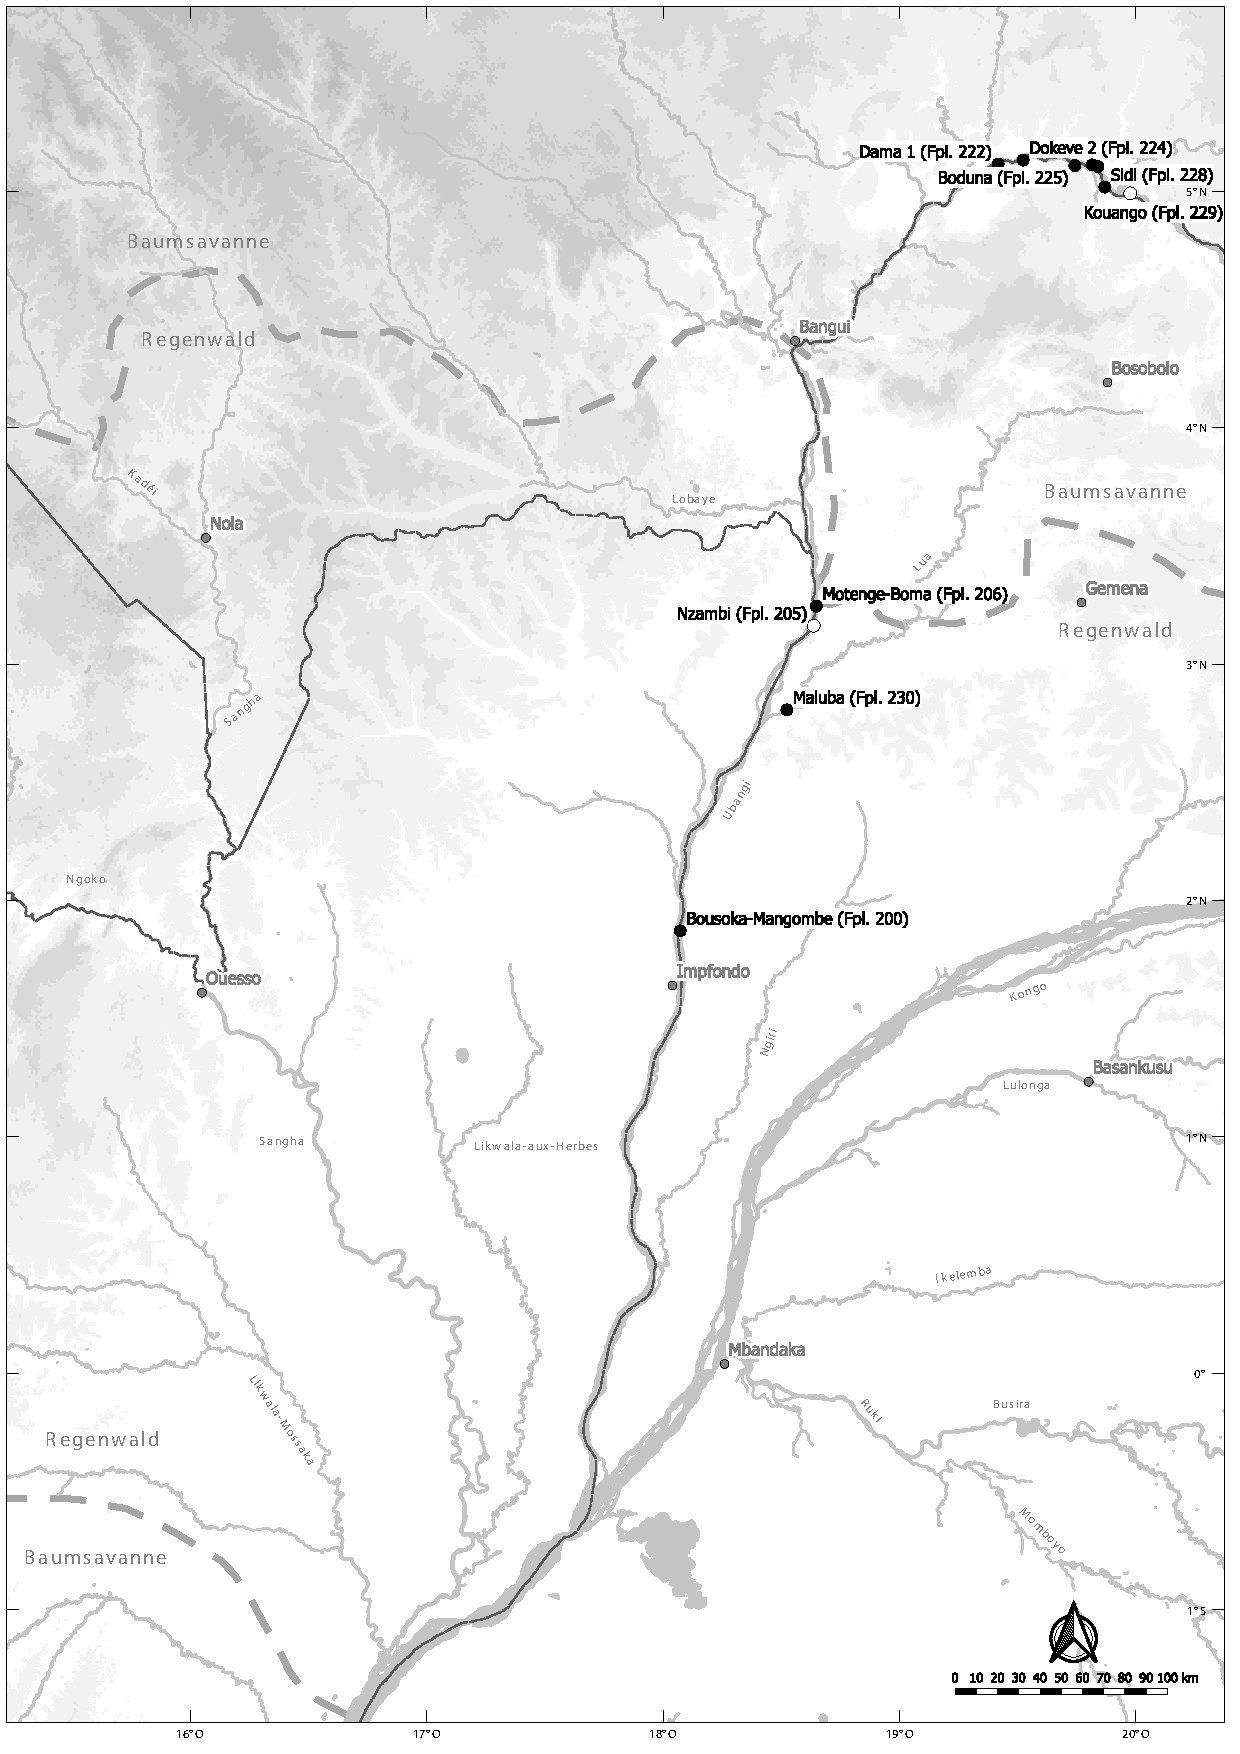
\includegraphics[width=\textwidth]{fig/DAM_Verbreitung.pdf}
	\caption{Dama-Gruppe: Verbreitung.}
	\label{fig:DAM_Verbreitung}
\end{figure*}

\paragraph{Formen}\hspace{-.5em}|\hspace{.5em}%
Bei 20~GE der Dama-Gruppe konnte die Gefäßform angesprochen werden. Neben stark rundbauchigen Gefäßen mit kurzem Hals (Typ D; 50\,\%; Abb.~\ref{fig:DAM_Typvertreter}.2, 6, 8) zeichnet sich die Stilgruppe durch flache Gefäße mit geschweifter Wandung, leichtem Zylinderhals und kurzen, ausbiegenden Rändern aus (Typ E; 45\,\%; Abb.~\ref{fig:DAM_Typvertreter}.1, 3, 4). Lediglich eine GE wurde als flaches Gefäß mit abknickender Wandung angesprochen (Typ F). Die GE der Dama-Gruppe zeigen eine deutliche Variabilität bei der Randgestaltung. Gerade abgestrichene Randlippen (M3; 26\,\%) kommen nur etwas häufiger vor als runde (M1; 22\,\%) oder gerillte Randabschlüsse (22\,\%). Die Ränder sind kurz konkav (B2; 23\,\%; Abb.~\ref{fig:DAM_Typvertreter}.1,3) oder gerade ausgbiegend (B1; 15\,\%; Abb.~\ref{fig:DAM_Typvertreter}.2). In geringerem Rahmen finden sich parallel aufsteigende (A1; 12), umgelegte (A2; 12\,\%), im Profil dreieckig verdickte (A2.3; 12\,\%) oder einbiegende Ränder (C1; 12\,\%). Nur in einzelnen Fällen ließen sich auch kurze konkav ausbiegende (B2.1; 8\,\%), verdickte (A4, 4\,\%) sowie konvex ausbiegende Ränder feststellen (B3; 4\,\%). Die Hälfte der GE zeigt einen konkav ausgearbeiteten Halsbereich, während der Schulterbereich entweder gerade oder konvex geformt ist. Der überwiegende Teil der GE zeigt lang ausgeführte Halsbereiche (89\,\%). Bei drei GE der Dama-Gruppe konnte die Bodenform angesprochen werden. Während eines der Gefäße aus Dama~I einen runden Boden aufweist (B1; Abb.~\ref{fig:DAM_Typvertreter}.3), ist der Boden des zweiten auffallend flach (B4; Abb.~\ref{fig:DAM_Typvertreter}.1).\footnote{Mit Blick auf die in Dama~I beobachtete Herstellung der beiden Gefäße durch Abformen in einer kleinen Erdkuhle könnte der flache Boden auch auf eine unbeabsichtigte Variation während des Herstellungsprozesses zurückgehen. Während des Töpferns wurde zu keinem Zeitpunkt die Ausarbeitung eines dediziert flachen Bodens beobachtet.} Eine dritte, aus Bousoka-Mangombe (Fpl.~200) stammende GE zeigt ebenfalls einen runden Boden (B1).

\paragraph{Verzierungen}\hspace{-.5em}|\hspace{.5em}%
Die Keramik der Dama-Gruppe zeichnet sich durch eine regelhafte Schnitzrouletteverzierung aus. Die verschiedenen Variationen machen zusammen 70\,\% der beobachteten Verzierungselemente aus. Daneben wurden fast ausschließlich horizontale Rillen beobachtet (Tab.~\ref{tab:Verzierungselemente}: 02.1; 28\,\%), die sich auf allen Gefäßteilen von der Innenseite der Ränder bis zum Gefäßbauch fanden (Anlage~4\subref{fig:DAM_Verz}). Daneben ließen sich lediglich in sehr geringen Anzahlen kleine, vertikale Eindrücke beobachten (Tab.~\ref{tab:Verzierungselemente}: 04.15; 2\,\%). Die Rouletteverzierung wurde regelhaft als einzelnes Band auf der Schulter oder dem Bauchbereich der Gefäße aufgebracht, seltener auch auf der Innenseite des Randes (Abb.~\ref{fig:DAM_Typvertreter}.4) oder außen am Rand (Abb.~\ref{fig:DAM_Typvertreter}.8). Die häufigste Schnitzroulette-Variante erzeugt ein \textit{erhabenes} rautenförmiges Muster (Tab.~\ref{tab:Verzierungselemente}: 21.7; 40\,\%), gefolgt von einer ganz ähnlichen Variante, bei der ein aus eingetiefeten Rauten bestehendes Muster entsteht (Tab.~\ref{tab:Verzierungselemente}: 21.10; 9\,\%). Das bei der Motenge-Boma-Gruppe (Kap.~\ref{sec:MTB-Gr}) häufige tannenbaumartige Schnitzroulette fand sich an den GE der Dama-Gruppe deutlich seltener (Tab.~\ref{tab:Verzierungselemente}: 21.12; 7\,\%). Ebenfalls beobachtet werden konnten Roulettes mit gezähnten tiefen Einschnitten (Tab.~\ref{tab:Verzierungselemente}: 21.5--6; 10\,\%) sowie eine komplexere, rautenförmige Muster erzeugende Variante (Tab.~\ref{tab:Verzierungselemente}: 21.8; 5\,\%). Anders als innerhalb der Motenge-Boma- (Kap.~\ref{sec:MTB-Gr}) sowie Kpetene-Gruppe (Kap.~\ref{sec:KPT-Gr}) wird bei der Dama-Keramik fast ausschließlich ein einzelnes horizontales Band im Schulterbereich in  Roulettetechnik aufgebracht. Flächige Muster lassen sich nicht beobachten. Die Unterteile und Standflächen der Dama-Gefäße sind durchweg unverziert (Anlage~4\subref{fig:DAM_Verz}).

\paragraph{Datierung}\hspace{-.5em}|\hspace{.5em}%
Die Keramik der Dama-Gruppe bildet das rezente keramische Spektrum am oberen \mbox{Ubangi} ab. Die Datierung des Materials basiert auf der Beobachtung der Herstellung dieser Keramik in Dama~I (Fpl.~222) sowie Sidi (Fpl.~228) bei den Prospektionen von 1985. Eine Scherbe, welche der Dama-Gruppe zugerechnet werden kann, wurde überdies bei der Grabung der Grube MLB~85/1-3-1 (Kat.-Nr.~1) in Maluba am Lua (Fpl.~230) im ersten Abtrag angetroffen.\footnote{Es ist auffällig, dass die entsprechenden Tafeln zeitgenössischer Keramik aus dem \textit{État Indépendant du Congo}, die sich im Besitz des damaligen \textit{Musée du Congo} befand \parencite[Taf.~XIV--XV]{Coart.1907}, keine rouletteverzierte Keramik aus dem Bereich des \mbox{Ubangi} zeigen.\label{ftn:Coart1907RouletteUbangi}}

\paragraph{Verbreitung}\hspace{-.5em}|\hspace{.5em}%
Die Keramik der Dama-Gruppe fand sich in einem nur vage eingrenzbaren Gebiet entlang des mittleren und oberen Laufes des \mbox{Ubangi} sowie des befahrenen Abschnitts des Lua (Abb.~\ref{fig:DAM_Verbreitung}). Eine dichte Belegung kann für das direkte Umfeld der drei Töpfereidörfer Dama~I (Fpl.~222), Boduna (Fpl.~225) und Sidi (Fpl.~228) beobachtet werden. Eine weitere Konzentration von der Dama-Gruppe zuordenbarer GE fand sich im Bereich des Lua und seiner Mündung in den \mbox{Ubangi}. Zwei GE fanden sich auch deutlich weiter südlich in Bousoka-Mangombe (Fpl. 200). Auffällig an diesem Verbreitungsgebiet ist, dass die Lücke zwischen den beiden im Fundgut beobachteten Hauptverbreitungsgebieten der Dama-Gruppe teilweise durch die Anwesenheit von Funden der ebenfalls rezenten Stilgruppen Mbati-Ngombe (Kap.~\ref{sec:MBN-Gr}; Abb.~\ref{fig:MBN_Verbreitung}) und Bangui (Kap.~\ref{sec:BAN-Gr}; Abb.~\ref{fig:BAN_Verbreitung}) aufgefüllt wird.